\documentclass[aspectratio=169]{beamer}

% Theme
\usetheme{Madrid}
\usecolortheme{default}

% Packages
\usepackage{graphicx}
\usepackage{tikz}
\usepackage{amsmath}
\usepackage{booktabs}

% Remove navigation symbols
\setbeamertemplate{navigation symbols}{}

% Add frame numbers
\setbeamertemplate{footline}[frame number]

% Title
\title{Fair District Maps\\Through Smart Computer Algorithms}
\subtitle{Edge-Weighted Recursive Bisection Explained}
\author{Giovanni Della-Libera}
\date{January 2026}

\begin{document}

% Title slide
\begin{frame}
\titlepage
\end{frame}

% Table of contents
\begin{frame}{What We'll Cover}
\tableofcontents
\end{frame}

% Section 1: The Problem
\section{The Redistricting Problem}

\begin{frame}{Why Do We Draw Congressional Districts?}
\begin{columns}
\column{0.5\textwidth}
\textbf{The Goal:}
\begin{itemize}
\item Every 10 years, new census
\item States get a certain number of representatives
\item Need to draw district boundaries
\item Each district $\approx$ 760,000 people (2020)
\end{itemize}

\vspace{1em}
\textbf{The Challenge:}
\begin{itemize}
\item Millions of possible ways to draw lines
\item Politicians often draw maps to favor their party
\item This is called \textbf{gerrymandering}
\end{itemize}

\column{0.5\textwidth}
% Placeholder for gerrymandering example image
\begin{center}
\fbox{\parbox{0.9\textwidth}{
\centering
\vspace{1cm}
Example:\\
Gerrymandered districts\\
can look very strange!\\
\vspace{1cm}
}}
\end{center}
\end{columns}
\end{frame}

\begin{frame}{What Makes a "Good" District Map?}
\textbf{Constitutional Requirements:}
\begin{enumerate}
\item \textbf{Equal Population}: Each district must have approximately the same number of people
\item \textbf{Contiguous}: Districts must be connected (you can walk from any part to any other part)
\end{enumerate}

\vspace{1em}
\textbf{Desirable Properties:}
\begin{itemize}
\item \textbf{Compact}: Districts should be reasonably circular/square, not weird snaking shapes
\item \textbf{Fair}: Maps shouldn't systematically favor one political party
\item \textbf{Transparent}: The process should be understandable and auditable
\end{itemize}

\vspace{1em}
\begin{center}
\textbf{Can we use math and computers to create better maps?}
\end{center}
\end{frame}

% Section 2: Graph Concepts
\section{Understanding Graphs}

\begin{frame}{What's a Graph? (Not the x-y kind!)}
\begin{columns}
\column{0.6\textwidth}
A \textbf{graph} is a way to represent connections:
\begin{itemize}
\item \textbf{Vertices} (nodes): The things we're connecting
\item \textbf{Edges}: The connections between them
\end{itemize}

\vspace{1em}
\textbf{For Redistricting:}
\begin{itemize}
\item Each \textbf{census tract} is a vertex
\item Census tracts that touch each other have an \textbf{edge}
\item Each vertex has a \textbf{weight} (population)
\end{itemize}

\column{0.4\textwidth}
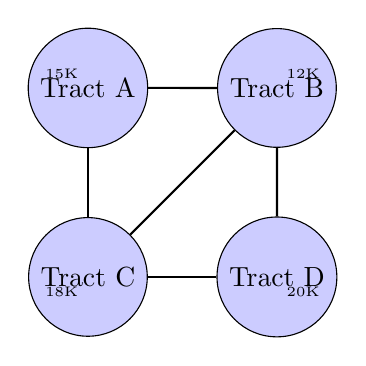
\begin{tikzpicture}[scale=1.2]
% Simple graph example
\node[circle,draw,fill=blue!20] (A) at (0,2) {Tract A};
\node[circle,draw,fill=blue!20] (B) at (2,2) {Tract B};
\node[circle,draw,fill=blue!20] (C) at (0,0) {Tract C};
\node[circle,draw,fill=blue!20] (D) at (2,0) {Tract D};

\draw[thick] (A) -- (B);
\draw[thick] (A) -- (C);
\draw[thick] (B) -- (D);
\draw[thick] (C) -- (D);
\draw[thick] (B) -- (C);

\node[above left] at (A) {\tiny 15K};
\node[above right] at (B) {\tiny 12K};
\node[below left] at (C) {\tiny 18K};
\node[below right] at (D) {\tiny 20K};
\end{tikzpicture}
\end{columns}

\vspace{1em}
\textbf{Key Insight:} Redistricting is a \textit{graph partitioning} problem—we need to split the graph into groups (districts) with equal total weight (population).
\end{frame}

\begin{frame}{From Real Geography to Graph}
\begin{columns}
\column{0.5\textwidth}
\textbf{Actual Census Tracts:}
\begin{itemize}
\item Small geographic areas
\item Typically 1,200-8,000 people
\item About 85,000 tracts nationwide
\item Shapes follow streets, rivers, etc.
\end{itemize}

\vspace{1em}
\textbf{Why Use Graphs?}
\begin{itemize}
\item Computers are great at graph problems
\item Preserves all geographic relationships
\item Automatically ensures contiguity
\end{itemize}

\column{0.5\textwidth}
% Placeholder for tract-to-graph visualization
\begin{center}
\fbox{\parbox{0.9\textwidth}{
\centering
\vspace{2cm}
Visual:\\
Census tracts\\
$\downarrow$\\
Abstract graph\\
\vspace{2cm}
}}
\end{center}
\end{columns}
\end{frame}

% Section 3: Recursive Bisection
\section{Recursive Bisection Algorithm}

\begin{frame}{The Basic Idea: Split in Half, Repeatedly}
\textbf{Recursive Bisection:} A "divide and conquer" approach
\begin{enumerate}
\item Start with the whole state
\item \textbf{Split it in half} (balanced by population)
\item Split each half in half
\item Keep going until you have the right number of districts
\end{enumerate}

\vspace{1em}
\begin{center}
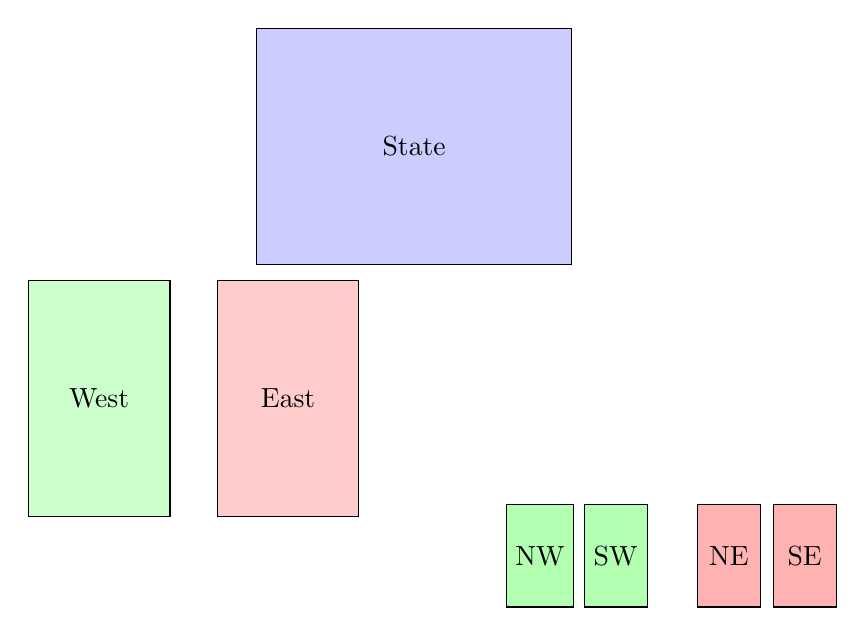
\begin{tikzpicture}[scale=0.8]
% Show 3 levels of splitting
\node[rectangle,draw,fill=blue!20,minimum width=4cm,minimum height=3cm] at (0,0) {State};

\pause
\node[rectangle,draw,fill=green!20,minimum width=1.8cm,minimum height=3cm] at (-5,-4) {West};
\node[rectangle,draw,fill=red!20,minimum width=1.8cm,minimum height=3cm] at (-2,-4) {East};

\pause
\node[rectangle,draw,fill=green!30,minimum width=0.8cm,minimum height=1.3cm] at (2,-6.5) {NW};
\node[rectangle,draw,fill=green!30,minimum width=0.8cm,minimum height=1.3cm] at (3.2,-6.5) {SW};
\node[rectangle,draw,fill=red!30,minimum width=0.8cm,minimum height=1.3cm] at (5,-6.5) {NE};
\node[rectangle,draw,fill=red!30,minimum width=0.8cm,minimum height=1.3cm] at (6.2,-6.5) {SE};
\end{tikzpicture}
\end{center}
\end{frame}

\begin{frame}{Example: 8 Districts = 3 Rounds of Splitting}
\begin{center}
\textbf{Round 1:} $1 \rightarrow 2$ regions\\
\textbf{Round 2:} $2 \rightarrow 4$ regions\\
\textbf{Round 3:} $4 \rightarrow 8$ districts

\vspace{2em}
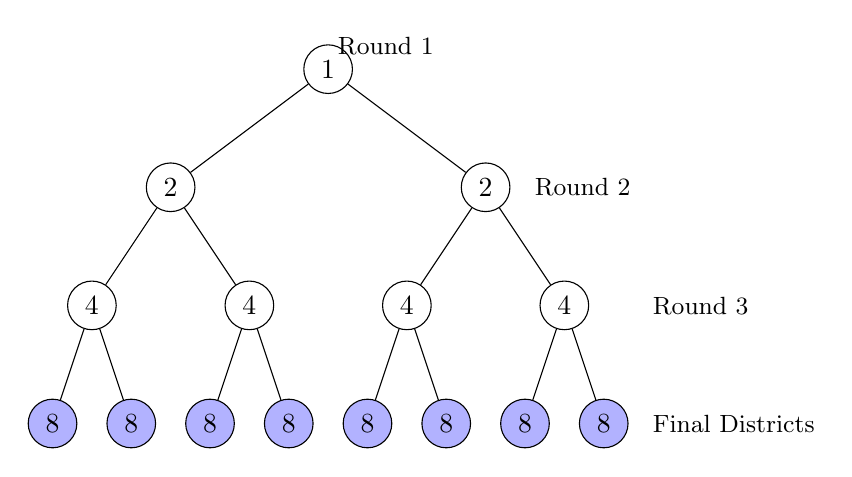
\begin{tikzpicture}
% Binary tree
\node[circle,draw] (root) at (0,0) {1};

\node[circle,draw] (left1) at (-2,-1.5) {2};
\node[circle,draw] (right1) at (2,-1.5) {2};

\node[circle,draw] (ll) at (-3,-3) {4};
\node[circle,draw] (lr) at (-1,-3) {4};
\node[circle,draw] (rl) at (1,-3) {4};
\node[circle,draw] (rr) at (3,-3) {4};

\node[circle,draw,fill=blue!30] (lll) at (-3.5,-4.5) {8};
\node[circle,draw,fill=blue!30] (llr) at (-2.5,-4.5) {8};
\node[circle,draw,fill=blue!30] (lrl) at (-1.5,-4.5) {8};
\node[circle,draw,fill=blue!30] (lrr) at (-0.5,-4.5) {8};
\node[circle,draw,fill=blue!30] (rll) at (0.5,-4.5) {8};
\node[circle,draw,fill=blue!30] (rlr) at (1.5,-4.5) {8};
\node[circle,draw,fill=blue!30] (rrl) at (2.5,-4.5) {8};
\node[circle,draw,fill=blue!30] (rrr) at (3.5,-4.5) {8};

\draw (root) -- (left1);
\draw (root) -- (right1);
\draw (left1) -- (ll);
\draw (left1) -- (lr);
\draw (right1) -- (rl);
\draw (right1) -- (rr);
\draw (ll) -- (lll);
\draw (ll) -- (llr);
\draw (lr) -- (lrl);
\draw (lr) -- (lrr);
\draw (rl) -- (rll);
\draw (rl) -- (rlr);
\draw (rr) -- (rrl);
\draw (rr) -- (rrr);

\node[right] at (0,0.3) {\small Round 1};
\node[right] at (2.5,-1.5) {\small Round 2};
\node[right] at (4,-3) {\small Round 3};
\node[right] at (4,-4.5) {\small Final Districts};
\end{tikzpicture}
\end{center}
\end{frame}

\begin{frame}{How Do We Actually Split?}
\textbf{We use a tool called METIS:}
\begin{itemize}
\item Specialized graph partitioning software
\item Developed at University of Minnesota
\item Used in engineering, scientific computing, etc.
\item Very good at splitting graphs efficiently
\end{itemize}

\vspace{1em}
\textbf{What METIS does at each split:}
\begin{enumerate}
\item Takes the current region (as a graph)
\item Finds a way to divide it into two parts
\item Makes sure each part has the right population
\item Makes sure each part is connected
\item Tries to minimize something (more on this next!)
\end{enumerate}
\end{frame}

% Section 4: The Key Innovation
\section{The Key Innovation: Edge Weights}

\begin{frame}{Baseline Approach: Treating All Connections Equally}
\textbf{Unweighted Recursive Bisection:}
\begin{itemize}
\item All edges are treated the same
\item METIS minimizes the \textbf{number of edges cut}
\item Doesn't care about boundary \textit{length}
\end{itemize}

\vspace{1em}
\begin{center}
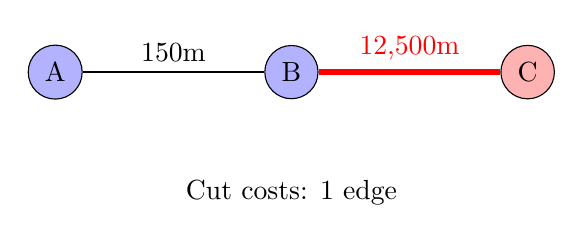
\begin{tikzpicture}[scale=1.5]
\node[circle,draw,fill=blue!30] (A) at (0,0) {A};
\node[circle,draw,fill=blue!30] (B) at (2,0) {B};
\node[circle,draw,fill=red!30] (C) at (4,0) {C};

\draw[thick] (A) -- node[above] {150m} (B);
\draw[thick,red,line width=2pt] (B) -- node[above] {12,500m} (C);

\node[below=0.5cm] at (2,-0.5) {Cut costs: 1 edge};
\end{tikzpicture}
\end{center}

\textbf{Problem:} Cutting between B and C adds 12.5 km of boundary!
\end{frame}

\begin{frame}{Our Innovation: Edge Weights Based on Real Length}
\textbf{Edge-Weighted Recursive Bisection:}
\begin{itemize}
\item Each edge has a \textbf{weight} = actual boundary length
\item METIS minimizes the \textbf{total weight of edges cut}
\item Directly minimizes total perimeter!
\end{itemize}

\vspace{1em}
\begin{center}
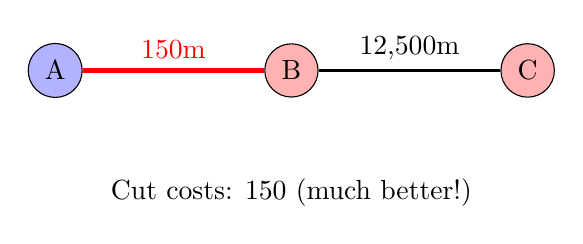
\begin{tikzpicture}[scale=1.5]
\node[circle,draw,fill=blue!30] (A) at (0,0) {A};
\node[circle,draw,fill=red!30] (B) at (2,0) {B};
\node[circle,draw,fill=red!30] (C) at (4,0) {C};

\draw[thick,red,line width=2pt] (A) -- node[above] {150m} (B);
\draw[thick] (B) -- node[above] {12,500m} (C);

\node[below=0.5cm] at (2,-0.5) {Cut costs: 150 (much better!)};
\end{tikzpicture}
\end{center}

\textbf{Insight:} METIS now strongly prefers to cut short boundaries, not long ones.
\end{frame}

\begin{frame}{Why Does This Matter?}
\textbf{Compact districts have shorter perimeters!}

\vspace{1em}
\begin{columns}
\column{0.5\textwidth}
\textbf{Circle:} Most compact shape
\begin{itemize}
\item Perimeter = $2\pi r \approx 6.28r$
\item Polsby-Popper score = 1.0
\end{itemize}

\column{0.5\textwidth}
\textbf{Squiggly shape:} Less compact
\begin{itemize}
\item Same area, much longer perimeter
\item Lower Polsby-Popper score
\end{itemize}
\end{columns}

\vspace{1em}
\textbf{By minimizing total perimeter, we automatically get more compact districts!}

\vspace{1em}
\begin{center}
\textit{Polsby-Popper formula:} $PP = \frac{4\pi \times \text{Area}}{\text{Perimeter}^2}$
\end{center}
\end{frame}

% Section 5: Examples
\section{Real Examples}

\begin{frame}{Minnesota: 8 Districts (Perfect Power of 2)}
\begin{columns}
\column{0.33\textwidth}

\includegraphics[width=\textwidth]{../../papers/03_combined_recursive_bisection/figures/minnesota_round_1_2_regions.png}
\begin{center}\small{Round 1: 2 regions}\end{center}

\column{0.33\textwidth}

\includegraphics[width=\textwidth]{../../papers/03_combined_recursive_bisection/figures/minnesota_round_2_4_regions.png}
\begin{center}\small{Round 2: 4 regions}\end{center}

\column{0.33\textwidth}

\includegraphics[width=\textwidth]{../../papers/03_combined_recursive_bisection/figures/minnesota_round_3_8_regions.png}
\begin{center}\small{Round 3: 8 districts}\end{center}
\end{columns}

\vspace{1em}
\textbf{Notice:} Each split creates two equal-sized regions. Final districts are compact with smooth boundaries.
\end{frame}

\begin{frame}{Alabama: 7 Districts (Not a Power of 2)}
\begin{columns}
\column{0.33\textwidth}

\includegraphics[width=\textwidth]{../../papers/03_combined_recursive_bisection/figures/alabama_round_1_2_regions.png}
\begin{center}\small{Round 1: 2 regions\\(4 vs 3)}\end{center}

\column{0.33\textwidth}

\includegraphics[width=\textwidth]{../../papers/03_combined_recursive_bisection/figures/alabama_round_2_4_regions.png}
\begin{center}\small{Round 2: 4 regions}\end{center}

\column{0.33\textwidth}

\includegraphics[width=\textwidth]{../../papers/03_combined_recursive_bisection/figures/alabama_round_3_7_regions.png}
\begin{center}\small{Round 3: 7 districts}\end{center}
\end{columns}

\vspace{1em}
\textbf{Notice:} Unequal splits (4-3, then 2-2-2-1). Algorithm handles this automatically! Still produces compact districts.
\end{frame}

\begin{frame}{Comparing Approaches: Minnesota Results}
\begin{center}
\begin{tabular}{lcc}
\toprule
\textbf{Method} & \textbf{Mean Polsby-Popper} & \textbf{vs Baseline} \\
\midrule
Baseline (Unweighted) & 0.288 & --- \\
\textbf{Edge-Weighted} & \textbf{0.468} & \textcolor{green}{+62\%} \\
Enacted 2020 Map & 0.287 & +0\% \\
\bottomrule
\end{tabular}
\end{center}

\vspace{1em}
\textbf{Takeaway:} Edge weights make a huge difference! Our algorithm produces more compact districts than both baseline and the actual enacted map.
\end{frame}

\begin{frame}{Comparing Approaches: Alabama Results}
\begin{center}
\begin{tabular}{lcc}
\toprule
\textbf{Method} & \textbf{Mean Polsby-Popper} & \textbf{vs Baseline} \\
\midrule
Baseline (Unweighted) & 0.246 & --- \\
\textbf{Edge-Weighted} & \textbf{0.369} & \textcolor{green}{+50\%} \\
Enacted 2020 Map & 0.297 & +21\% \\
\bottomrule
\end{tabular}
\end{center}

\vspace{1em}
\textbf{Takeaway:} Even with 7 districts (odd number), edge-weighted bisection produces compact districts that beat the enacted map!
\end{frame}

% Section 6: National Results
\section{National Results}

\begin{frame}{Results Across All 50 States}
\begin{center}
\textbf{All 435 Congressional Districts (2020 Census)}
\end{center}

\vspace{1em}
\begin{tabular}{lcc}
\toprule
\textbf{Method} & \textbf{Mean PP} & \textbf{Improvement} \\
\midrule
Baseline Recursive Bisection & 0.235 & --- \\
\textbf{Edge-Weighted Bisection} & \textbf{0.367} & \textcolor{green}{+56\%} \\
Enacted 2020 Districts & 0.305 & +30\% \\
\bottomrule
\end{tabular}

\vspace{1em}
\textbf{Key Results:}
\begin{itemize}
\item \textbf{37 of 50 states}: Our algorithm beats enacted maps
\item \textbf{Partisan-drawn states}: Biggest improvements
  \begin{itemize}
  \item Illinois: +174\%
  \item Louisiana: +104\%
  \item New Hampshire: +102\%
  \end{itemize}
\end{itemize}
\end{frame}

\begin{frame}{Why This Matters}
\textbf{Advantages of Algorithmic Redistricting:}

\begin{enumerate}
\item \textbf{Objectivity}: No human bias or political manipulation
\item \textbf{Transparency}: Anyone can run the algorithm and verify results
\item \textbf{Reproducibility}: Same inputs always produce same outputs
\item \textbf{Compactness}: Automatically produces compact districts
\item \textbf{Speed}: Runs in minutes, not months
\end{enumerate}

\vspace{1em}
\textbf{Limitations:}
\begin{itemize}
\item Doesn't consider communities of interest
\item Doesn't try to create competitive districts
\item Pure geography-based approach
\end{itemize}

\vspace{1em}
\textbf{Use Case:} Provides a \textit{neutral baseline} to measure gerrymandering
\end{frame}

% Conclusion
\section{Conclusion}

\begin{frame}{Summary}
\textbf{What We Learned:}
\begin{enumerate}
\item Redistricting can be viewed as a \textbf{graph partitioning problem}
\item \textbf{Recursive bisection}: Split in half repeatedly until we have enough districts
\item \textbf{Edge weights}: Using real boundary lengths dramatically improves compactness
\item \textbf{METIS}: Powerful tool that does the hard work of finding good partitions
\item Works for both even (Minnesota, 8) and odd (Alabama, 7) district counts
\end{enumerate}

\vspace{1em}
\textbf{The Big Idea:}\\
By encoding geographic information (boundary lengths) into the graph, we can automatically create compact, fair districts without any human intervention.
\end{frame}

\begin{frame}{Questions?}
\begin{center}
\Large{\textbf{Thank You!}}

\vspace{2em}
For more details:
\begin{itemize}
\item Full paper: \texttt{papers/03\_combined\_recursive\_bisection/}
\item Code: \texttt{github.com/yourusername/redistricting}
\item Interactive maps: Visit our web dashboard
\end{itemize}
\end{center}
\end{frame}

\end{document}
